\section{Implementación}
\label{s3:sec:Implementacion}


\subsection{FPGA}
\label{s3:subsec:fpga}
Para la implementación del juego sobre la FPGA, se ha decidido implementar
distintos módulos, conectados entre ellos, que permiten calcular el estado
del juego. La relación entre los distintos módulos se peude ver en la
figura~\ref{s3:fig:componentes-fpga-a}. Además, para que el juego pueda
funcionar a una velocidad adecuada, pero se pueda comunicar con los
maletines, y además pintar en el monitor vga, cada módulo está controlado
por su propio reloj, como se explica en la sección~\ref{s3:subsubsec:clocking}
y se muestra en la figura~\ref{s3:fig:componentes-fpga-clocking}. 


\begin{figure}[h]
\todo{Revisar la parte del teclado, me he inventado un poco, y me he comido
  el controlador}.\\
\todo{No se si esto es muy pequeño y habría que separarlo, o incluso mover
  la imagen de clocking a la sección correspondiente o no}
\centering
\begin{subfigure}{.5\textwidth}
  \centering
  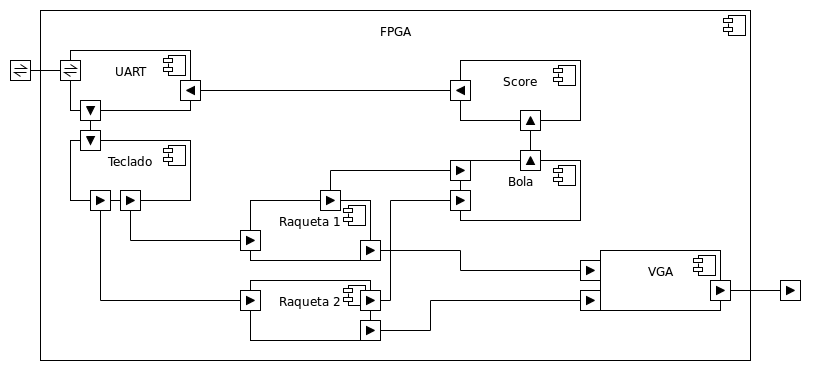
\includegraphics[width=1.0\textwidth]{images/fpga_componentes.png}
  \caption{Componentes implementados.}
  \label{s3:fig:componentes-fpga-a}
\end{subfigure}%
\begin{subfigure}{.5\textwidth}
  \centering
  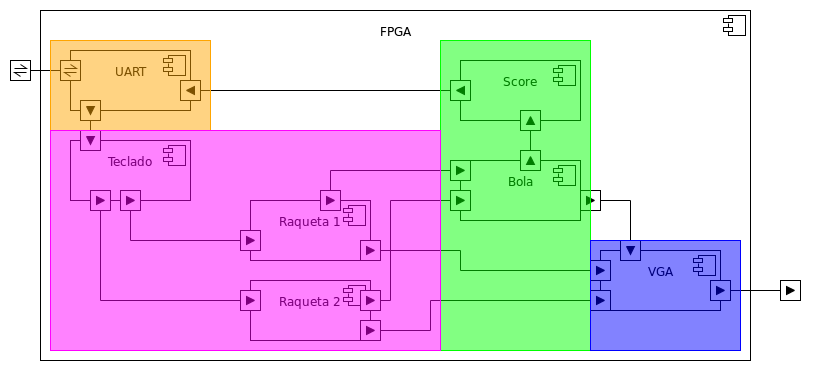
\includegraphics[width=1.0\textwidth]{images/fpga_componentes_timing.png}
  \caption{Distintos relojes utilizados.}
  \label{s3:fig:componentes-fpga-clocking}
\end{subfigure}
\caption{Diagrama de componentes implementados en la FPGA. }
\label{s3:fig:componentes-fpga-a}
\end{figure}

Como se muestra en la figura, los módulos de los que está compuesta la
implementación sobre la FPGA son:
\begin{itemize}
\item \emph{Módulo UART:} módulo encargado de leer y enviar información a
  través de la UART de la FPGA. Posee señales de control para indicar
  cuándo un dato se ha recibido, o cuando está ocupada enviando
  información.
\item \emph{Módulo teclado:} traduce la información recibida por la UART a
  comandos internos entendidos por el juego. Este diseño nos permite
  desacoplar el módulo teclado de la UART, y cambiarlo por otros módulos
  que interpreten otros dispositivos de entrada, como puede ser un teclado
  PS2.
\item \emph{Módulo raquetas:} contienen la información de la posición de
  las raquetas. Las teclas leídas del módulo teclado modifican la posición
  de este módulo. Este módulo se encuentra instanciado varias veces, una
  por cada raqueta del juego.
\item \emph{Módulo bola:} calcula en cada pulso del reloj del juego la
  nueva posición de la pelota. Además, recibe la información de las palas
  para calcular los rebotes con ellas, o si un jugador gana el partido
  actual. Si es el caso, el módulo informa al módulo de puntuaciones para
  registrar el evento.
\item \emph{Módulo puntuación:} encargado de guardar la información de los
  partidos. Cuando un jugador consigue un tanto, se comunica con el módulo
  de la UART para enviar la información a los maletines.
\item \emph{Módulo VGA:} a partir de la información del módulo bola, y de
  los módulos de raquetas, dibuja en un monitor VGA el juego. \rev{Si da
    tiempo, el diagrama de flujo que controla este módulo viene definido
    en la figura bla bla bla}.
\end{itemize}

\subsubsection{Gestión de los relojes}
\label{s3:subsubsec:clocking}

\todo{Escribir, haciendo referencia a la
  figura~\ref{s3:fig:componentes-fpga-clocking}. Quizás aquí sea
  interesante mencionar el tema de la sincronización y la necesidad de
  utilizar biestables para mantener la diferencia entre relojes.}

\subsection{Maletines ARM}
\label{s3:subsec:maletines}
\todo{Escribir esto, haciendo referencia a~\ref{s3:fig:FSM_maletin}. Si se
  decide mover la imagen a~\ref{s2:subsec:sistema-entero}, inventarse que
  poner. }\\
\todo{Sería interesante explicar lo del tecldo, y lo que se  hace para
  poder conectar varios maletines en serie.}

\begin{figure}[h]
  \centering
  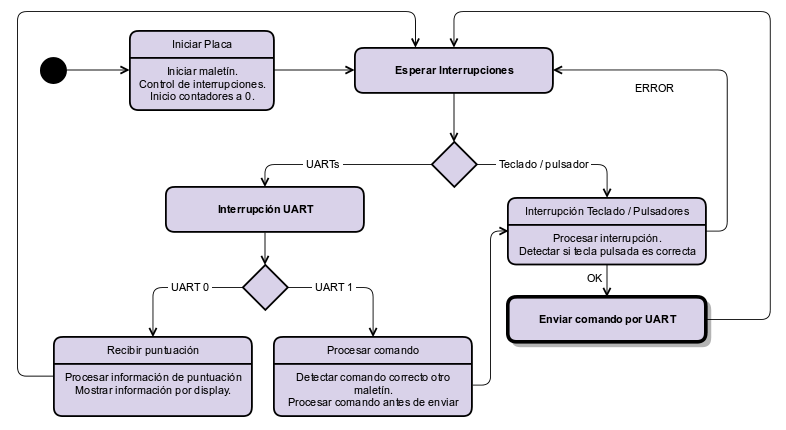
\includegraphics[width=1.0\textwidth]{images/maletin_fsm.png}
  \caption{FSM describiendo el comportamiento de los maletines.}
  \label{s3:fig:FSM_maletin}
\end{figure}





%
%
%%%
%%% Local Variables:
%%% mode: latex
%%% TeX-master: "../main.tex"
%%% End:


